\documentclass[preprint]{sigplanconf}

% The following \documentclass options may be useful:
%
% 10pt          To set in 10-point type instead of 9-point.
% 11pt          To set in 11-point type instead of 9-point.
% authoryear    To obtain author/year citation style instead of numeric.

\usepackage{amsmath}
\usepackage{graphicx}
\usepackage{subfigure}
\usepackage{algorithmic}
\usepackage{algorithm}

\begin{document}

\conferenceinfo{PLDI'11}{June 4-8, San Jose, California.} 
\copyrightyear{2011} 
\copyrightdata{[to be supplied]} 

\titlebanner{preprint}        % These are ignored unless
\preprintfooter{}   % 'preprint' option specified.

\title{Debugging by \textit{lastChange}}
\subtitle{}

\authorinfo{Salman Mirghasemi\and Claude Petitpierre}
           {Ecole Polytechnique F\'ed\'erale de Lausanne}
           {\{salman.mirghasemi,claude.petitpierre\}@epfl.ch}

\authorinfo{John J. Barton}
           {IBM Research - Almaden}
           {johnjbarton@johnjbarton.com}

\maketitle

\begin{abstract}
Backward search from bug symptoms to defects-which cause the bug-is a natural way to debugging. However, due to the lack of support for easily bakward movement by  traditional debugging approaches (e.g., breakpoint-based or log-based debugging), applying this strategy-if it is not pracatically impossible-demands a lot of effort from developers. Tracking origins to wrong values is a fundumental step in this process and any aid in this regard can greatly reduce the complexity of debugging for developers.

To address this problem, we propose a new functionality in debuggers, \textit{lastChange}, which locates the last place a value is changed and lets developer to collect data and ask for more \textit{lastChange} queries at the located point. Although \textit{lastChange} algorithm is based on program re-execution, contrary to other replay-based algorithms which require exactly the same re-executions, it only requires bug reproduction by re-executions. In other words \textit{bug reproduciblity} (i.e., a test case is available which reproduces the bug) is the only prerequisite for \textit{lastChange} functinality.

As a proof of concept, we developed \textit{Querypointer}, a prototype which enhances Firebug JavaScript debugger with \textit{lastChange} feature. Moreover, \textit{Querypointer} provides mechanisms for automated bug reproduction, and a novel user interface to investigated execution points and results.

\end{abstract}

\category{D.2.5}{Testing and Debugging}{Debugging aids}
\category{D.2.6}{Programming Environments}{Integrated environments}

\terms
Algorithms, Human Factors, Languages

\keywords
LastChange, Locating Defects, Breakpoint, Watchpoint, Logging

%---------------------------------------------------------------------------------------------------
\section{Introduction}
Debugging is an inevitable part of programming, still hard and time-consuming. To fix a bug, developers have to reproduce and monitor the buggy execution several times to understand the program's unexpected behavior. Trial and error, guess-work and analyzing huge collected data are the inseparable parts of this process. According to \cite{LaToza}, developers spend about fifty percent of their time debugging. Therefore, every improvement to debugging techniques and tools can considerably save developers' time and improve programs' quality.

Locating defects cause the bug is the main part of debugging. A common strategy for locating defects is starting from bug symptoms and backward movement by following the origings to wrong values. While this strategy seems straightforward and effective, applying this strategy using traditional methods is complicated. There are two traditional approaches to debugging, breakpoint-based and log-based debugging. None of these approaches assist developer in finding origings to a wrong value. It is due to developer to search source files, find the list of possible origings to a wrong value and set breakpoints or insert log statements in a way that covers all possible origins.

The next dilemma is data collection. In breakpoint debugging, developer has to memorize values or manually collect data at every breakpoint hit. As the number of breakpoint hits increases, the process of checking the program state, collecting data and resuming the execution becomes cumbersome. While in breakpoint-based debugging, the whole program state is available to developer, in log-based debugging, developer has to decide about data should be collected when inserts the log statement. It is very common that developer has to repeat this step several times due to insufficient collected data. Once the adequate data is collected, it still requires analysis and understanding. Developers usually end up in dealing with long log files and analyzing huge collected data.

Our proposal is a new functionality in debuggers which locates the origin of a wrong value, call it \textit{lastChange}. The only prerequisite for \textit{lastChange} functionality is bug reproduciblity (i.e., there is a test case which reproduces the bug). Assume that the program execution is paused on a breakpoint and the developer is suspicious about the value of an object property or variable. The developer selects \textit{lastChange} on the value and it is due to debugger to locate and shows the last change of object property or variable. Debugger reproduces the buggy execution and collects limited data and once the execution reaches the same place (i.e., the same breakpoint hit), call it \textit{reproduction point}, it pauses the execution, analyzes the collected data and shows the location of the last change to the developer. Developer can also examine the program state at the located point of execution, and ask for a new \textit{lastChange} at this point.

Our contribution in this paper is the algorightm \textit{lastchange}, which locates the last place a value is changed, gathers other values from that execution point, and allows \textit{lastChange} operations from that point. The algorithm builds on existing breakpoint debugger technology. We demonstrate the feasibiltily of the algorithm with \textit{Querypointer}, an implementation extending the Firebug JavaScript debugger. \textit{Querypointer} also provides mechanism for automated bug reproduction, and a centralized user interface which summarizes investigated execution points and collected results. 

The rest of the paper is organized as follows. First, we demonstrate the \textit{lastChange} usage on a simple example with the comparison to breakpoint debugging. Section 3 presents \textit{lastChange} algorithm. In section 4, we explain the details of the JavaScript prototype implementation. 

%---------------------------------------------------------------------------------------------------
\section{Introductory example}

We illustrate the \textit{lastChange} functionality by a simple
example. The example demonstrates a buggy JavaScript code in a HTML
page (Figure ~\ref{fig:js-code}). The page contains a button (line 40)
showing the value of \texttt{myObject.myProperty}.  When the user
clicks on the button, the \texttt{onClick} function (line 13) is
called. This function increases the value of
\texttt{myObject.myProperty} by one (line 15) and calls
\texttt{updateButton} function which updates button's text to the new
value (line 22).  Once the page is loaded for the first time the
button shows \texttt{1} as the initial value of
\texttt{myObject.myProperty}.  In practice when the user clicks on the
button, \texttt{0} appears instead of \texttt{2}: there is a bug.

Two other functions are called in \texttt{onClick()}, \texttt{foo()}
and \texttt{bar()}. As developers we often encounter function calls
which seem perpheral to our current concern; they may have been added
by another developer, or we may have forgotten their exact properties
or those properties may have changed, and so on. The difference
between what we expect these functions to do, e.g. nothing
interesting, and what they do in practice may cause bugs.

To start debugging, the developer sets a breakpoint
on line 22 and once the button is clicked execution is paused at line
22. Figure ~\ref{fig:example1} shows the Firebug debugger while the
execution is paused. Firebug has several panels (e.g., HTML, CSS,
Script, DOM, etc.) that each demonstrate one aspect of the Web page.
The Script panel contains the list of all loaded source
files and regular debugging facilities such as setting breakpoints and
stepping. To the right of the script panel, the Watch panel shows the program state
where the developer can examine object and variable values. In our case, the
\texttt{myObject.myProperty} value at the paused point is zero. We expected this value to be \texttt{2}.

\begin{figure}[htp]
\begin{verbatim}
1 <html>
...
5   <script type="text/javascript">
6    myObject = {myProperty : 1};
7    myCondition = {value : 1};
...
13   function onClick(){
14     foo();
15     myObject.myProperty++;
16     bar();
17     ...
18     updateButton();
19   }
20   function updateButton(){
21     var myParagraph =
          document.getElementById("myButton");
22     myButton.innerHTML = myObject.myProperty;
23   }   
24   function foo(){
25  	 myCondition.value = oldValue;
26   }  
27   function bar(){ 
28     if (!myCondition.value)
29         myObject.myProperty = 0;
30   }
31  </script> 
...
40  <button id="myButton" onclick="onClick()">
41  	1 
42  </button>
43 </html>
\end{verbatim}
\caption{A Web page containing JavaScript code. Some lines not related to our paper have been elided.}
\label{fig:js-code}
\end{figure}


\begin{figure}[htp]
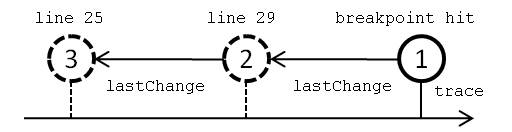
\includegraphics{5-example-points.jpg}
\caption{The examinated points before locating the defect.}
\label{fig:example-points}
\end{figure}

To apply backward search strategy for locating defects, the developer
first needs to know the origin to the wrong value. To achieve this
goal using breakpoints, the developer should search code to find and
set breakpoint at all possible places that
\texttt{myObject.myProperty} might get a new value.  However, an
object and property can be accessed and changed through different
names and methods. There is no simple way to identify these alias or
even their total number.  The developer can make a good guess and set
breakpoints on lines where the property seems to be changed. Then they
re-execute the program and examine the state looking for values that
may lead to the incorrect value observed at line 22. All this work
must be repeated if a new alias is discovered or if the some
information related to the buggy result was missed while stopped on
one of the breakpoints.

In contrast, we propose a high-level function in debugger,
\textit{lastChange}, which provides the answer without tedious manual
effort from the developer. By right clicking on
\texttt{myObject.myProperty} in the Watch panel, the developer can run
\textit{lastChange} command (Figure ~\ref{fig:example2}). Debugger
re-executes the program and halts again at the breakpoint on line 22.
However, it shows a new QP panel, centered on the source at line 29
(Figure ~\ref{fig:example3}), the point of \testit{lastChange}.  To
the right, the TraceData panels shows values of properties from the
program state when it passed through line 29.  These two panels
resemble the Script and Watch panels, but they show data collected by
the debugger at an execution point which has now past: these are
'traces' or 'logs' of information collected during the re-execution.

\begin{figure*}[htp]

\subfigure[A screen shot of the Firebug debugger while running the example code from Fig.~\ref{fig:example2}. The Script
  panel is selected; it gives access to
  all loaded source files and allows breakpoints to be set on lines. In this
  figure, the execution is paused at line 22 by a regular
  breakpoint. The Watch panel at the right shows the program state at
  the paused
  point. ]{\label{fig:example1}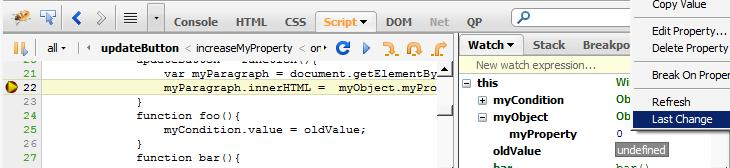
\includegraphics[width=1.0\textwidth,
    height=.19\textheight]{1-bp22.jpg}}

\subfigure[Developer can query \textit{lastChange} on a value by right-clicking 
on the
  value of \texttt{myProperty}.]{\label{fig:example2}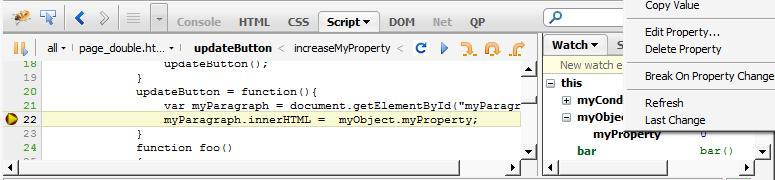
\includegraphics[width=1.0\textwidth,
    height=.19\textheight]{2-bp22-lastChange.jpg}}

\subfigure[The result of \textit{lastChange} query for
  \texttt{myObject.myProperty}. The left panel, QP, shows the source
  code at the point of \textit{lastChange}; The right panel,
  TraceData, shows the collected data at the
  point.]{\label{fig:example3}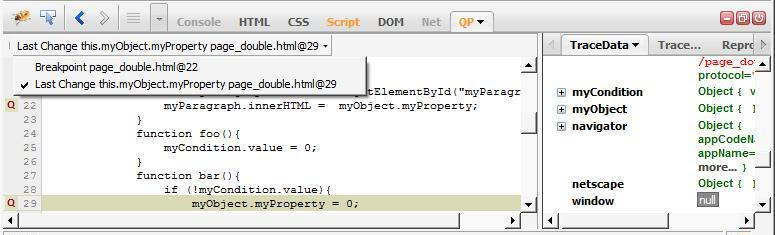
\includegraphics[width=1.0\textwidth,
    height=.23\textheight]{3-lastChange.jpg}}

\subfigure[The result of \textit{lastChange} query for
  \texttt{myCondition.value}. The opened list on the top of the left
  panel shows the visited execution points. Clicking on each point in
  the list shows the corresponding code and
  data.]{\label{fig:example4}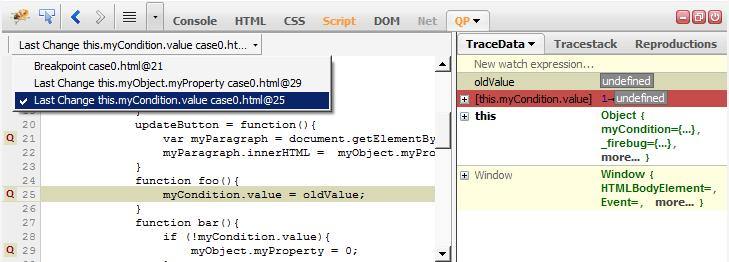
\includegraphics[width=1.0\textwidth,
    height=.23\textheight]{4-lastChange2.jpg}}

\caption{The stages of locating the defect using \textit{lastChange} feature.}
\label{fig:lastChange}
\end{figure*}

Looking at line 29, it seems that something is wrong with
\texttt{myCondition.value} which causes line 29 execution. The
developer examines \texttt{myCondition.value} and it is
\texttt{undefined}. The next step is to know when this property got
this value. To do so, the developer runs \textit{lastChange} command
on \texttt{myCondition.value} at this point. Debugger re-executes the
execution and pauses at the reproduction point and shows line 25-the
place \texttt{undefined} value is assigned to
\texttt{myCondition.value} (Figure ~\ref{fig:example3}). Now it is
clear that the bug occurs because \texttt{oldValue} is
\texttt{undefined} once execution reaches line 25.

As demonstrated in Figure ~\ref{fig:example-points}, the developer
examinated three points of execution. The first point was the breakpoint set by the developer.
The second and third points preceded the breakpoint in time.
All three points-the history
of the search for the defect-are available through the debugger's
interface. On the top of the left panel in Figure ~\ref{fig:example3}
there is an opened list which shows all three examinated points. The
first one is the breakpoint on line 22, the second one is the point
which is the last change of \texttt{myObject.myProperty} before the
reaching the breakpoint and finally the last one is the point of
execution in which \texttt{myCondition.value} gets the
\texttt{undefined} value. Moreover, the source lines related to these
points are tagged with red-cycle icons.

Notice that in our example, \textit{lastChange} combines some aspects
of breakpoint and of log-based debugging. Like breakpoint debugging,
the developer re-executes a live runtime without changing the source
and without a special execution environment beyond the debugger. The
state of the program memory and the call stack are available at the
lastChange point. Like log-based debugging, the program state and the
call stack are recorded during program execution. We can't halt the
program at \textit{lastChange} because we don't know which is the last
one until we return to the original breakpoint. (In section 5 we
discuss cases were it is possible to pause at lines of \textit{lastChange}).

%---------------------------------------------------------------------------------------------------
\section{\textit{lastChange} Algorithm}

The story starts when developer examines the program state at a breakpoint hit and asks for the \textit{lastChange} of a value. The \textit{lastChange} algorithm is based on program re-execution. Therefore it is assumed that the execution can be reproduced automatically (e.g., by a given test case) or with the developer's assistance. The breakpoint hit becomes the \textit{reproduction point}. Debugger sets hooks on all instructions that might be the result of \textit{lastChange} query, re-executes the program, at every hook hit, \textit{change event}, collects limited data and once the execution reaches the reproduction point, it analyzes the collected data and shows the result. The result is a partial snapshot of the program state at the execution point that last change occured. 

As we shown in the previous section, a \textit{lastChange} query can be performed on the result of another \textit{lastChange} query. If we name the reproduction point \textit{R}, we can write the first \textit{lastChange} in the introductory example in this form: \textit{lastChange(R, myObject.myProperty)}. It means that this query is defined at \textit{R}. If we name the result of this query \textit{A}, we can write the second \textit{lastChange} in this form: \textit{lastChange(A, myCondition.value)}. In this way, a sequence of \textit{lastChange} queries with any length can be defined.

\textit{lastChange} can be called on two different types of values: An object property or a variable value. In JavaScript, every available variable in a frame comes from one of the scopes in the frame's scope chain. There are five different scope types: global, local, with, catch, closure. We explain each case separately.

\subsection{\textit{lastChange} on object propery}
To simplify the algorithm explanation and avoid technical details, we assume two basic operations and later we explain the details of this two operations. The first opertion is \texttt{objectId()} which gets a JavaScript object and returns an integer as its identifier. This identifier is unique for every object during one execution. The second operation is \texttt{setPropertyChangeHook()} which gets function as the callback and a string as the property name like \texttt{foo}. Whenever property \texttt{foo} in any object changes the callback will be called. The callback function receives a reference to the owner of \texttt{foo}.


\begin{figure}[htp]
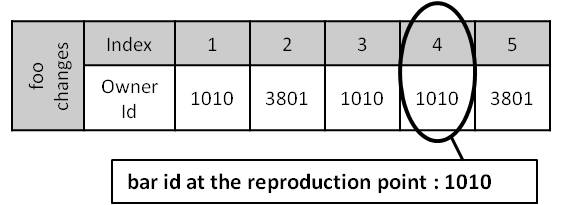
\includegraphics[width=.48\textwidth]{6-foo-changes1.jpg}
\caption{The list of property \texttt{foo} change events and \texttt{bar} id at the reproduction point which identifies the last change of \texttt{bar.foo} in the list. Column 3 is also a change of the object we want to study, id 1010, but it is not the last change; Column 5 is also a change of a property \texttt{foo} but its not for the object we are interested in.}
\label{fig:foo-changes1}
\end{figure}

Once developer asks for the last change of \texttt{bar.foo} at the reproduction point, debugger calls \texttt{setPropertyChangeHook()} with \texttt{foo} as the property name and re-executes the program. Whenever \texttt{foo} changes and the callback function is called, debugger first calls \texttt{objectId()} on the \texttt{foo} owner object. Then it stores owner id and stack frame locations. The reason we keep object id instead of a reference to the object itself is to let garbage collector to destroy dead objects. Whenever the execution reaches the reproduction point it looks at the history of \texttt{foo} changes and finds the last \texttt{foo} change with the same object id as \texttt{bar} id at the reproduction point. Figure ~\ref{fig:foo-changes1} shows the list of property \texttt{foo} change events in a hypothetical execution. \texttt{bar} id at the reproduction point is 1010, so the last change of \texttt{bar.foo} is the forth column.

\subsubsection{\texttt{objectId()}}
The object id is kept as a property of the object, \texttt{\_objectid}, which is not enumerable. Therefore, it will not appear in \texttt{for(property in object)} loops and has no effect on the executing program. Once \texttt{objectId()} is called on an object and the object has not \texttt{\_objectId} property, this property is defined by calling \texttt{defineProperty} JavaScript function. As a parameter it can be specified that the defined property is not enumerable. Then it is enough to assign a new generated id to this property.

\subsubsection{\texttt{setPropertyChangeHook()}}
To implement this operation, we use two features that are available in Firefox JavaScript engine. First, every regular JavaScript object has a \texttt{watch()} function which receives two parameters, a property name and another function as a callback. Whenever the property with the given name changes the calleback function is called. The hook is set by this function is enabled even if the property is removed and added again [ref]. The issue with this function is that it can only be applied to available objects. However, at the beginning of re-execution there is no object available. To solve this issue we use the second feature. Enabling a flag gives us the place the object created including the JavaScript file url and line number (e.g., myFile.js, line 24). Though this is a limited data, it helps us to get a reference to the object once it is created. Then it is enough to set objet id and call \texttt{watch()} with the property name. In section 4.1, we explain how we get reference to the created objects.
 
\subsection{\textit{lastChange} on variable} 
In JavaScript, every frame has a scope chain and every available variable in the frame comes from one of the scopes in the frame's scope chain. Once developer asks for the last change of variable \texttt{foo} at the reproduction point, debugger first determines the variable's scope as follows: it iterates over the scopes in the scope chain and the first scope which has a variable with the same name is the variable's scope. There are five different scope types: local, global, \texttt{with}, closure, \texttt{catch}. We explain these cases in two groups.


\subsubsection{global and \texttt{with} scopes}
Global scope is the the most outer scope in the scope chain and it is also refered as global object which is usually \texttt{window} object. This scope is a regular JavaScript object and therefore every global variable is a property of global object. Similar to global scope, \texttt{with} scopes are also regular objects. A \texttt{with} scope is created by a \texttt{with()} block with an object as the parameter. Every property of passed object is available inside the block as a variable. Debugger treats the case where variable's scope is global or \texttt{with}, like \textit{lastChange} on an object property. 

\subsubsection{local, closure and \texttt{catch} scopes}
Local scope refers to the most nested scope in the scope chain. Closure scope refers to the scope which is created once a function is defined. Catch scope is the scope created in the catch block of try-catch statements and contains the exception variable. These scopes are not necessarily regular JavaScript objects. Therefore, to track changes to a variable in these scopes we use a different strategy. 

\begin{figure}[htp]
\begin{verbatim}
10  function parent(){
11    var var1;
12    var1 = ...;
13    function myfun(){
14      var1 = ...;
15      function firstChild(){
16       	var var1;
17        var1 = ...;
18      }  
19      function secondChild(){
20        var1 = ...;			      
21      }
22    }  
23  }    
\end{verbatim}
\caption{Sample JavaScript code demonstrating local and clousure variables.}
\label{fig:js-closure}
\end{figure}

A variable in these types of scope can only be changed in the function the variable is defined or the nested fuctions. For example in Figure ~\ref{fig:js-closure}, variable \texttt{var1} in line 11 can only be changed in lines 10 to 23. Therefore, after locating the function in which the variable is defined, it is enough to parse the code inside the function block and set a hook on all lines where the variable is assigned a new value.% TODO lines or instruction???
We also set a hook at the first line of the function which is corresponding to the line variable is defined. In Figure ~\ref{fig:js-closure}, if the execution is paused at line 17 and the last change of \texttt{var1} is queried, two hooks on lines 16 and 17 will be set, but if the execution is paused at line 20 , four hooks on lines 11, 12, 14, 20 will be set. These two cases are different due the fact that \texttt{var1} in \texttt{firstChild} is a local variable but in \texttt{secondChild} is a closure variable.

Everytime one of the hooks hits a new change event is inserted to the list of change events. During execution the same variable might be changed several times but in different scopes. Figure ~\ref{fig:recursive} demonstrates one case that a scope identifier is necessary for locating the right answer. In this case the same variable \texttt{x} is changed several times but in different scopes due to the recursive calls. Without the scope id calling \textit{lastChange(x)} at point C will return point B while the right answer is point A.

\begin{figure}[htp]
\begin{verbatim}

  function f(){
    var x;
    x++;
    f();
  }

Sample Trace:

   f()
A  |  x changes; 
   |  f()
   |  |  x changes;
   |  |  f()
B  |  |  |  x changes; 
C  |  ?

\end{verbatim}
\caption{A recursive call trace demonstrates the need for scope id. Querying \textit{lastChange} on \texttt{x} at point C should return point A not B.}
\label{fig:recursive}
\end{figure}

\begin{figure}[htp]
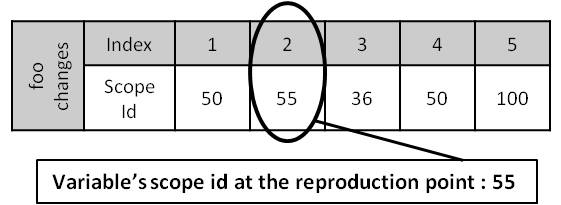
\includegraphics[width=.48\textwidth]{7-foo-changes2.jpg}
\caption{The list of variable \texttt{foo} change events and the \texttt{foo}'s scope id at the reproduction point which identifies the last change.}
\label{fig:foo-changes2}
\end{figure}

The scope id is kept as a variable in the scope, \texttt{\_scopeId}. As we said, a hook is set on the first instruction of the function defines the variable. Whenever this hook hits,  \texttt{\_scopeId} variable is set by \texttt{eval()} function. For example evaluating \texttt{var \_scopeId = 50} will create a variable with name \texttt{\_scopeId} and value \texttt{50} in the local scope.
 
\subsection{\textit{lastChange} on \textit{lastChange}}
The algorithm we explained so far needs an enhancement to support longer sequence of \textit{lastChange}s. We explain first the issue and then the solution. Consider the following points:

\begin{center}
\textit{
 point A : the reproduction point \\
 point B : lastChange(A, bar.x) \\
 point C : lastChange(B, baz.y) 
 }
 \end{center}
According to the algorithm explained in the previous section none of the points B and C can be identified before reaching point A. Therefore, all \texttt{x} changes for piont B and all \texttt{y} changes for point C are stored. Once the execution reaches point A, and the exact \texttt{bar} id reveals, point B can be identified among the change events in the history of \texttt{x} changes. The problem arises in recognizing point C. To recognize point C, we need \texttt{baz} id at point B, but B is a past program state, and \texttt{baz} id has not been collected at this point. 

To address this issue, debugger does a dependency analysis between all \textit{lastChange} queries and computes the additional data required to be collected at each point. For example in the mentioned case, \texttt{baz} id- if it is available- should be collected at all points \texttt{x} changes. Having this additional data, locating point C, using \texttt{baz} id at point B is straightforward (Figure ~\ref{fig:lastchange-lastchange}).

\begin{algorithm}
\caption{\textit{lastChange} queries dependency analysis.}
\label{dependency-analysis}
\begin{algorithmic}

\FOR{$q$ in $queries$} 
 \FOR {$p$ was defined at the $q$ result}
   \IF {$p$ is a lastChange on object property} 
     \STATE property id should be stored at $q$ change events. 
   \ELSIF {$p$ is a lastChange on variable} 
     \STATE variable scope id should be stored at $q$ change events.
	 \ENDIF 
 \ENDFOR 
\ENDFOR

\end{algorithmic}
\end{algorithm}

\begin{figure}[htp]
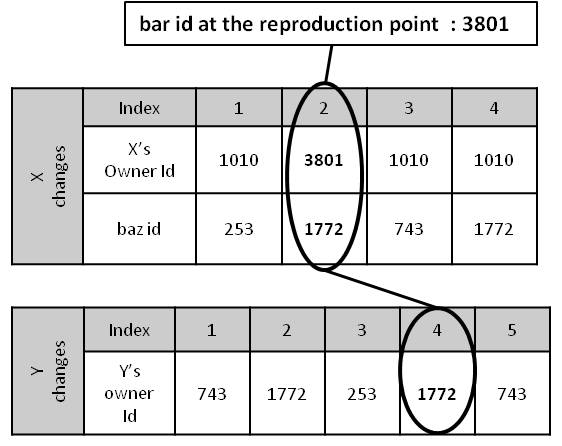
\includegraphics[width=.48\textwidth]{8-lastchange-lastchange.jpg}
\caption{The list of change events stored for locating point B, the \textit{lastChange} of \texttt{bar.x} at the reproduction point, and point C, the \textit{lastChange} of  \texttt{baz.y} at point B.}
\label{fig:lastchange-lastchange}
\end{figure}




%---------------------------------------------------------------------------------------------------
\section{JavaScript implementation}
The JavaScript prototype is implemented as an extension to Firebug[] javasrcipt debugger. 

\subsection{Tracking object creation}
Now we discuss two mentioned assumptions. In the standard JavaScript every object has a \texttt{watch()} function which receives two parameters, a property name and another function as a hook. Whenever the property with the given name changes the hook function is called. The issue with using this function is that it can only be applied to available objects. However, at the beginning of re-execution there is no object available. To solve this issue we use a feature in Firefox JavaScript engine, setting a flag gives us the place the object created (e.g., myFile.js, line 24). Though this is a limited data it can help us to get a reference to the object once it is created. Therefore, at the reproduction point, debugger gets the creation location of \texttt{bar} and once the execution reaches to that location it gets a reference to the created object and sets a unique id for it.

\subsection{Execution reproduction}
Altough execution reproduction is basicly should be provided by the developer, we tried to devise some automatic way which reproduces the execution. In the prototype, develooper can choose among three reproduction options. The first one is using a test case which provided by developer. The second one is by record and replay and the third one is local-reproduction.

Two parts should be carefully considered in execution reproduction. First, the initial state should be the same as previous execution. Second, the similar actions and events should be applied to the program during the execution. In the record and replay approach, debugger stores the initial page url and user actions and during replay phase, opens the same url and emulates user actions. 
In the local reproduction approach, debugger calls the funtion on the bottom of stack with the same parameters.

\subsection{Data collection}

\subsection{User interface}

\section{Converting \textit{lastChange} result to a conditional breakpoint}
We believe that in many cases it is possible to convert the \textit{lastChange} result to a conditional breakpoint and therefore debugger is able to pause at the point
 instead of showing collected data to the developer. Here, we present an example which shows a case this transformation is not possible.

Figure ~\ref{fig:counter-example} shows a function with processes an array. The array contains numbers except one itme which is \texttt{undefined} and it causes a bug in line 30. There is a call to \texttt{randomPermutation} function in line 11 which randomly permutates the array item. So at every execution the \texttt{undefined} item will be in a new place. Calling \textit{lastChange} on \texttt{x} at the place bug happens, gives a point which shows line 14. Although this point exists at every re-execution but it can not be identified by a conditional breakpoint. 

\begin{figure}[htp]
\begin{verbatim}
10 function randomProcess(array){
11   randomPermutation(array);
12   var x, y;
13   for (var i=0 ; i<array.length ; i++){
14      x = array[i]
...
30      y = x+1;
31   }
32 }
\end{verbatim}
\caption{A counter-example for transforming \textit{lastChange} to a conditional breakpoint.}
\label{fig:counter-example}
\end{figure}
 

%\section{}
%---------------------------------------------------------------------------------------------------
\section{Reproducible Non-deterministic Execution}
Thus far we have not discussed problems caused by mul-tiple threads or other sources of non-deterministic execu-tions. We want to explain why we believe \textit{lastChange} is robust in the practically important case where a bug is reproducible even though the execution may not be deterministic. 
Because \textit{lastChange} require re-execution, we rely on reproducible but not necessarily deterministic execution. A bug is reproducible for a developer when the developer can start from a determined initial state, operate on the program with a list of actions, and reproduce the symptoms of the bug. The details of the execution can change each time we re-execute the buggy program, but the buggy result is the same. The entire query chain reapplies during each execution so the data we show the developer will be internally consistent. The reproducibility of the bug means that the defect is very unlikely to depend on the order of events during the execution.

In this important case of reproducible bugs, \textit{lastChange} are more effective than breakpoints. In the case of logically deterministic program execution, we can use the result from a \textit{lastChange} operation to set a conditional breakpoint then re-execute the program to position the execution trace backwards from our first breakpoint. %(This may be a useful adjunct for Querypoint debuggers to implement, but this backwards motion in the execution logic is not required for Querypoint debugging.) Thus in this case Querypoint debugging can do the same kinds of things as conventional breakpoints just more automatically.

In the case of a non-deterministic program, a \textit{lastChange} is not equivalent to any series of conventional watchpoints or breakpoints. Each time we re-execute a non-deterministic program, the details of execution in-struction order may change. For example, if we record the source code lines every time a conventional watchpoint hits, the record may differ each time we re-execute. Sup-pose we consult one such record and set a breakpoint on the last entry, the apparent lastChange source line. When we re-execute, the breakpoint will hit, but the information we gain may be incorrect: this may not be the lastChange for this particular re-execution. The \textit{lastChange} method records the values we need and the sequence of source lines from all of the watchpoints, then analyzes the record to select the correct lastChange point. The data shown to the developer will be internally consistent, but of course it may change from a previous re-execution, surprising the developer. This is just a signal that the execution is not deterministic. In future we hope to compare queries from successive executions as a tool for learning about non-deterministic executions.

\section{Evaluation}

\section{Related Work}

\textit{lastChange} functionality supports obtaining information about the execution state logically earlier in the control flow. This support resembles a mixture of replay-based and logging-based debugging. Replay-based approaches capture limited data during execution and replay the bug-gy execution to reach past points. In contrast, logging-based approaches collect enough data during execution to relieve developer from re-execution. Replay-based approaches impose much less runtime overhead (about two orders of magnitudes) comparing to logging-based appproches. However, developer has to re-execute the buggy execution several times. \textit{lastChange} functionality collects data on re-execution but this data is limited to the current queries of developer.

Among replay-based debuggers we compare to bdb \cite{Boothe} and reverse watchpoint \cite{Maruyama}.  A bidirectional C debugger, bdb employs a step counter to locate the requested point from the beginning of execution. It relies on deterministic execution replay (i.e., the same sequence of instructions in re-execution) and records the results of non-deterministic system calls and re-injects them into the program when it is replayed. It makes use of checkpoints to reduce the time needed for re-execution.  Reverse watchpoint, is proposed by Maruyama et al., analyses the execution and moves the debugger to the last write access of a selected variable by re-executing the program from the \cite{Maruyama}.  Similar to bdb it relies on deterministic replay and uses a counter to correctly locate a point in the next execution. The main disadvantage of these appraoches is requiring the exactly the same executions. Even one instruction difference between in two executions leads to wrong results. This requirement is that much restricting that after ten years from bdb paper publication, there is no newer implementation of this idea. On the other hand, \textit{lastChange} doesn't require any special feature in the re-rexecution and it is fit to everyday's developers' debugging practice. 

Among logging-based approaches are "omniscient" debuggers ODB\cite{Lewis} and Unstuck[]. Omniscient debuggers have been proposed as a solution for the problems of breakpoint-debugging. Both approaches keep the log history in memory and hence can only record and store the complete history for a short period of time. These debuggers record all the events that occur during the buggy execution and later let the developer to navigate through the obtained execution log. In this approach there is no execution to resume: moving backwards in the log can be similar to moving forwards. Omniscient debuggers suffer from a different set of issues. First, the recording step is time expensive and it should be repeated in case of changes in program. Second, the execution log cannot fully replace the live execution. There are other aspects of execution (e.g., program user interface, file system, database tables, etc.) which are also important in debugging and are not available to the developer in omniscient debuggers. Third, querying collected data (e.g., to restore the program state at a certain point) may not be efficient enough for debugging of realistic programs.

A more scalable approach has been proposed by Pothier et al. \cite{Pothier}. Their back-in-time debugger, TOD, addresses the space problem by storing execution events in a distributed database. Comparing to Omniscient debuggers our approach is lightweight and more flexible. Developer can start debugging just after reproducing bug without a capturing step.  Changing inputs or environment settings and re-executing to investigate the bug works as in conventional breakpoint debuggers.

Two new directions in logging debuggers explore more detailed use of the log and more effective logging approaches. WhyLine\cite{Ko} provides visual interface to collected runtime information and let developer to move  on execution log using queries expressed in terms of the programming objects. WhyLine stores the program user in-terface in addition to program trace and provides answers to why and why not questions to the user. Jive\cite{Czyz} depicts the history of execution by a sequence diagram and lets user to query on events database. Both tools suffer from similar issues with omniscient debuggers; 
%both provide models for extending Querypoint debugging to obtain a better user interface while retaining the flexible conven-tional replay model of debugging.  

A recent work by Lienhard et al.\cite{Lienhard} suggests virtual machine level support for keeping the object flow. It rep-laces every object reference with an alias object which keeps the history of changes to the object reference. In this way, when an object is collected by garbage collector, its track of changes (if it is not referenced by other alias-es) will be also collected. Though this approach incurs less runtime overhead (7 times to 115 times) in comparison to omniscient debuggers, it adds memory overhead. Querypoint debugging uses re-executions to gather infor-mation requested by the developer: the memory overhead depends on the query not the entire program. Moreover, the Lienhard et al. debugger significantly changes the virtual machine, while our approach is a generalization to conditional breakpoints and available debugger infrastructure can be adapted to support it. 
 
\textit{lastChange} functionality does rely on a conventional breakpoint to begin queries, a requirement not shared by full logging solutions.  Here we leverage past experience of developers, but there are also new tools [] to help with this problem in the case of graphical and event based systems.


\section{Conclusions and Future Work}



% We recommend abbrvnat bibliography style.

\bibliographystyle{abbrvnat}

% The bibliography should be embedded for final submission.

\begin{thebibliography}{10}
\softraggedright

\bibitem[Bond(2007)]{Bond}
M.D. Bond, N. Nethercote, S.W. Kent, S.Z. Guyer, and K.S. McKinley. \newblock Tracking bad apples: reporting the origin of null and undefined value errors.
\newblock In \emph{22nd annual ACM SIGPLAN conference on Object-oriented programming, systems, languages, and applications(OOPSLA)},
October, 2007.

\bibitem[Boothe(2000)]{Boothe}
B. Boothe. \newblock Efficient algorithms for bidirectional debugging.
\newblock In \emph{Conference on Programming Language Design and Implementation(PLDI)},
June, 2000.

\bibitem[Czyz(2007)]{Czyz}
J.K. Czyz, and B. Jayaraman. \newblock Declarative and visual debugging in Eclipse.
\newblock In \emph{OOPSLA workshop on eclipse technology eXchange},
October, 2007.

\bibitem[Ko(2008)]{Ko}
A.J. Ko, and B.A. Myers. \newblock Debugging reinvented: asking and answering why and why not questions about program behavior.
\newblock In \emph{30th international conference on Software engineering(ICSE)},
May, 2008.

\bibitem[LaToza(2006)]{LaToza}
T.D. LaToza, G. Venolia, and R. DeLine. \newblock Maintaining mental models: a study of developer work habits
\newblock In \emph{28th international conference on Software engineering(ICSE)},
May, 2006.

\bibitem[Lewis(2003)]{Lewis}
B. Lewis, and M. Ducasse. \newblock Using events to debug Java programs backwards in time.
\newblock In \emph{Companion of the 18th annual ACM SIGPLAN conference on Object-oriented programming, systems, languages, and applications(OOPSLA)},
2003.

\bibitem[Lienhard(2008)]{Lienhard}
A. Lienhard, T. G\^{\i}rba, and O. Nierstrasz. \newblock Practical Object-Oriented Back-in-Time Debugging.
\newblock In \emph{22nd European conference on Object-Oriented Programming(ECOOP)},
July, 2008.

\bibitem[Maruyama(2003)]{Maruyama}
K. Maruyama, and T. Kazutaka. \newblock Debugging with Reverse Watchpoint.
\newblock In \emph{Proceedings of the Third International Conference on Quality Software},
2003.

\bibitem[Pothier(2007)]{Pothier}
G. Pothier, \'{E}. Tanter, and J. Piquer. \newblock Scalable omniscient debugging.
\newblock In \emph{22nd annual ACM SIGPLAN conference on Object-oriented programming, systems, languages, and applications(OOPSLA)},
October, 2007.


\end{thebibliography}

\end{document}
